 \documentclass{beamer}
%
% Choose how your presentation looks.
% For more themes, color themes and font themes, see:
% http://deic.uab.es/~iblanes/beamer_gallery/index_by_theme.html
%
\mode<presentation>
{
  \usetheme{Madrid}      % or try Darmstadt, Madrid, Warsaw, ...
  \usecolortheme{seahorse} % or try albatross, beaver, crane, ...
  \usefonttheme{serif}  % or try serif, structurebold, ...
  \setbeamertemplate{navigation symbols}{}
  \setbeamertemplate{caption}[numbered]
  \setbeamertemplate{itemize/enumerate body begin}{\large}
\setbeamertemplate{itemize/enumerate subbody begin}{\large}
\setbeamertemplate{itemize/enumerate subsubbody begin}{\large}

  \usepackage{amsmath}
  \usepackage{tcolorbox}
  \usepackage[export]{adjustbox}
  \tcbuselibrary{most}
  \usepackage{arydshln}
  \usepackage{tikz}
  \usetikzlibrary{plotmarks}
  \usepackage{pgfplots}
 %\usepackage{enumitem}
%\usepackage{enumerate}
  %\usepackage[shortlabels]{enumitem}
} 


\definecolor{myblue}{RGB}{65,105,225} 
\definecolor{myorange}{RGB}{250,190,0}

\setbeamercolor{structure}{fg=white,bg=myorange}
\setbeamercolor*{palette primary}{fg=myblue,bg=myorange}
\setbeamercolor*{palette secondary}{fg=white,bg=myblue}
\setbeamercolor*{palette tertiary}{bg=myblue,fg=white}
\setbeamercolor*{palette quaternary}{fg=white,bg=myorange!50}

\setbeamercolor{frametitle}{fg=black!90!myblue}

\setbeamercolor{section in head/foot}{fg=white,bg=myblue}
\setbeamercolor{author in head/foot}{fg=black,bg=myorange}
\setbeamercolor{title in head/foot}{fg=white,bg=myblue}

\setbeamertemplate{navigation symbols}{}

\setbeamertemplate{itemize/enumerate body begin}{\large}
\setbeamertemplate{itemize/enumerate subbody begin}{\large}


\defbeamertemplate*{headline}{mytheme}
{%
  \begin{beamercolorbox}[ht=2.25ex,dp=3.75ex]{section in head/foot}
    \insertnavigation{\paperwidth}
  \end{beamercolorbox}%
}%

\defbeamertemplate*{footline}{mytheme}
{
  \leavevmode%
  \hbox{%
  \begin{beamercolorbox}[wd=.5\paperwidth,ht=2.25ex,dp=1ex,right]{author in head/foot}%
    \usebeamerfont{author in head/foot}\insertshortauthor\hspace*{2em}
  \end{beamercolorbox}%
  \begin{beamercolorbox}[wd=.5\paperwidth,ht=2.25ex,dp=1ex,left]{title in head/foot}%
    \usebeamerfont{title in head/foot}\hspace*{2em}\insertshortsubtitle\hspace*{2em}
    \insertframenumber{} / \inserttotalframenumber
  \end{beamercolorbox}}%
  \vskip0pt%
}

\usepackage[english]{babel}
%\usepackage[utf8x]{inputenc}
\usepackage{xcolor}
\usepackage{listings}
\usepackage{pgf}  
\usepackage{textpos}
\usepackage{tabulary}
\usepackage{scrextend}
\usepackage{hyperref}
\usepackage{setspace}
\usepackage{rotating}
\lstset
{
    language=[LaTeX]TeX,
    breaklines=true,
    basicstyle=\tt\scriptsize,
    %commentstyle=\color{green}
    keywordstyle=\color{blue},
    %stringstyle=\color{black}
    identifierstyle=\color{magenta},
}
\newcommand{\bftt}[1]{\textbf{\texttt{#1}}}
%\newcommand{\comment}[1]{{\color[HTML]{008080}\textit{\textbf{\texttt{#1}}}}}
\newcommand{\cmd}[1]{{\color[HTML]{008000}\bftt{#1}}}
\newcommand{\bs}{\char`\\}
\newcommand{\cmdbs}[1]{\cmd{\bs#1}}
\newcommand{\lcb}{\char '173}
\newcommand{\rcb}{\char '175}
\newcommand{\cmdbegin}[1]{\cmdbs{begin\lcb}\bftt{#1}\cmd{\rcb}}
\newcommand{\cmdend}[1]{\cmdbs{end\lcb}\bftt{#1}\cmd{\rcb}}

\newcommand{\wllogo}{\textbf{Overleaf}}

% this is where the example source files are loaded from
% do not include a trailing slash
\newcommand{\fileuri}{https://raw.githubusercontent.com/GiancarloSucci/UniBo.IDSEPC.A2022/main/A2022.IDSEPCLaTeX/}


\usepackage{stackengine}
\def\Ruble{\stackengine{.67ex}{%
  \stackengine{.48ex}{\textsf{P}}{\rule{.8ex}{.12ex}\kern.6ex}{O}{r}{F}{F}{L}%
  }{\rule{.8ex}{.12ex}\kern.6ex}{O}{r}{F}{F}{L}\kern-.1ex}



%----------------------------------------------------------------------------------------
%	TITLE PAGE
%----------------------------------------------------------------------------------------
\title[L04]{Artificial Intelligence, Blockchain, e Criptovalute nello Sviluppo Software \newline\newline
Lezione 6: Distributed Cognition, Extended Mind, and Systemic Thinking} % The short title appears at the bottom of every slide, the full title is only on the title page

\author[{\tiny Giancarlo Succi }]{Giancarlo Succi\\\\ Dipartimento di Informatica -- Scienza e Ingegneria\\Universit\`{a} di Bologna\\
\bftt{g.succi@unibo.it}
} % Your name
\institute[unibo] % Your institution as it will appear on the bottom of every slide, may be shorthand to save space


\date{} % Date, can be changed to a custom date

\setbeamertemplate{navigation symbols}{}
\AtBeginSection[]
{
        \begin{frame}<beamer>{Outline}
                \tableofcontents[currentsection]
        \end{frame}
}
\begin{document}

\begin{frame}
\titlepage % Print the title page as the first slide

\end{frame}

%=============================================

\addtobeamertemplate{frametitle}{}{%
\begin{textblock*}{10mm}(-0.01mm,-0.95cm)

\includegraphics[width=0.9cm]{unibo-logo.png}
\end{textblock*}}

%=============================================


\begin{frame}
{\centerline{Structure of the lecture}}
\begin{itemize}
    \item Extended Mind
    \item Distributed Cognition
    \item Systemic Thinking
    \end{itemize}
\end{frame}

\begin{frame}
{\centerline{Boundaries of the Mind}}

\begin{center}
\begin{itemize}
    \item Where is our mind?
    \begin{itemize}
    \item Are the hands part of our mind?
\end{itemize} 
\end{itemize} 

 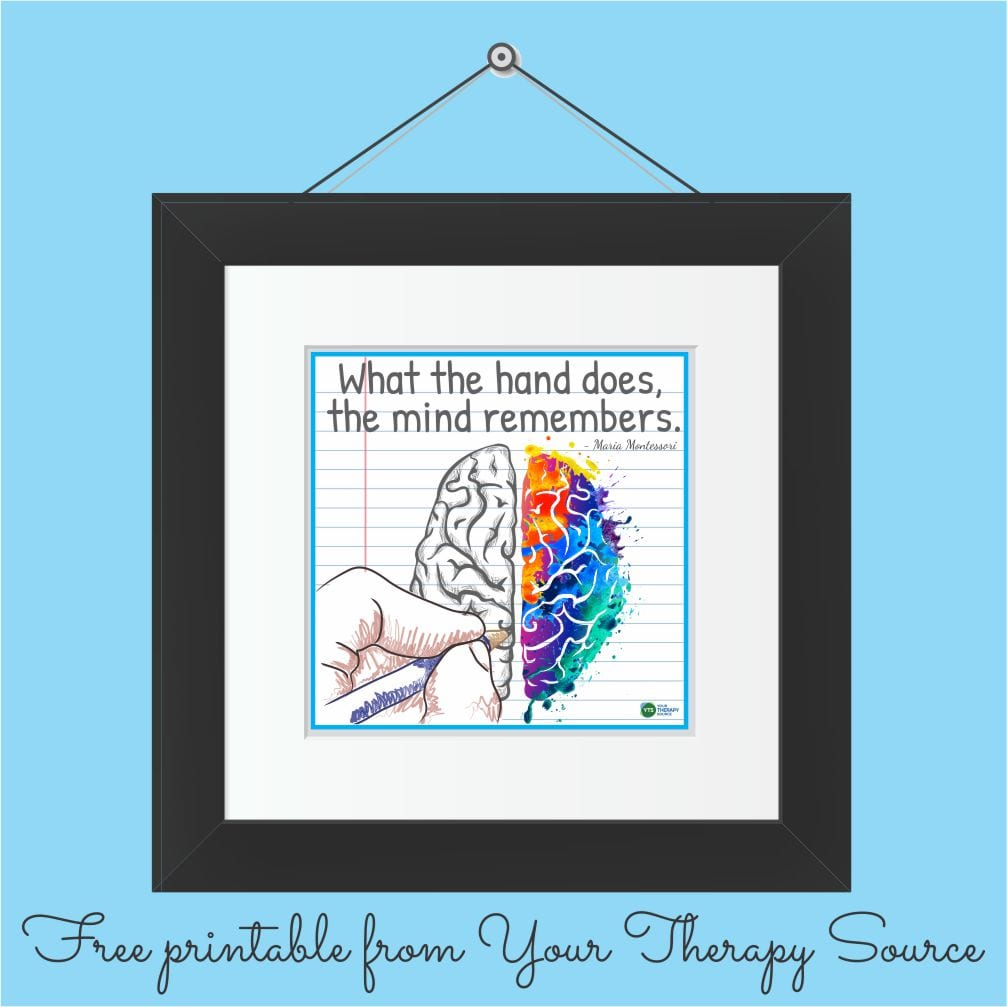
\includegraphics[width=5cm]{P2023.AIBCCSS.ExtendedMindDistributedCognitionSystemicThinking/what-the-hand-does-the-mind-remembers.jpg}
 
 \end{center}

\begin{center}
\tiny
Reference: Robert MacDougall, ``The Significance of the Human Hand in the Evolution of Mind,'' The American Journal of Psychology, 16(2):232 -- 242, Apr., 1905\\Picture taken from \url{https://www.yourtherapysource.com/blog1/2019/02/07/3-evidence-based-benefits-of-writing-by-hand/}.
\end{center}
\end{frame}


\begin{frame}
{\centerline{Extended Mind (1/2)}}

\begin{itemize}
    \item Let us consider a simple problem: we are given shapes and we have to see if they fit holes:
\end{itemize} 

\begin{center}
 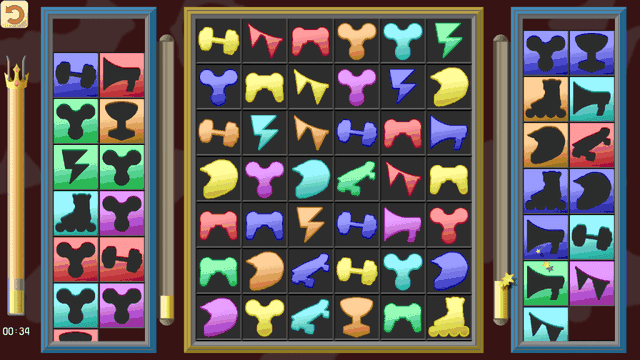
\includegraphics[width=8cm]{P2023.AIBCCSS.ExtendedMindDistributedCognitionSystemicThinking/campaignlevel-3-f53c.png}
 
 \end{center}

\begin{center}
    \tiny{Source of the content: Andy Clark and David Chalmers, ``The extended mind,'' Analysis 58 (1): 7--19 , 1998 \\Picture taken from \url{https://gurugamer.com/mobile-games/shapes-and-holes-a-new-mobile-puzzler-where-you-fit-things-into-other-things-1214}.}
\end{center}
\end{frame}


\begin{frame}
{\centerline{Extended Mind (2/2)}}
\begin{itemize}
    \item Let us consider three cases:
    \begin{itemize}
        \item this is a computer game (as in the picture) and the person has to rotate the pieces by mind and determines the fitting;
        \item this is a paper game and the person has pieces that s/he rotates manually to determine the fit;
        \item let us assume that the person has an implanted device, say, special smart glasses, that perform the rotation and then s/he just does the fitting
    \end{itemize}
    \item What is the level of cognition present in these cases?
        \begin{itemize}
   		 \item Clark and Chalmers claim that it is the same.
        \end{itemize}
    \item Therefore, what is the boundary of our mind?
\end{itemize} 
\begin{center}
    \tiny{Source of the content: Andy Clark and David Chalmers, ``The extended mind,'' Analysis 58 (1): 7--19 , 1998}
\end{center}

\end{frame}

\begin{frame}
{\centerline{Tools and Mind}}
\begin{itemize}
    \item There are many tools even before computer that helped our cognitive tasks
    \begin{itemize}
        \item abacus
        \item paper and pen
        \item sliding rule
        \item $\ldots{}$
            \end{itemize}
    \item Once we start using it, they become intrinsic part of our reasoning and computational process
    \item Think at how we do computations in column
           \begin{itemize}
        		\item papers and pen are essential components of our reasoning process
		\item even when we do the computation in our mind we often simulate the presence of paper and pen
	   \end{itemize} 
    \item Once more, \textcolor{orange}{\bf what are the boundaries of our mind}?
\end{itemize} 

\begin{center}
    \tiny{Source of the content: Andy Clark and David Chalmers, ``The extended mind,'' Analysis 58 (1): 7--19 , 1998}
\end{center}

\end{frame}

\begin{frame}
{\centerline{Impact}}
\begin{itemize}
    \item We care about this for at least three reasons:
    \begin{itemize}
        \item we understand that the request of tools may be not a caprice of a spoiled kid but an actual desire to organize the (extended) mind in the most effective way
        \item when developing tools we need to think at how such tools can most effectively ``extend'' the mind of the users, and not simply being tools
        \item when creating a (development) environment for us and for our people we must determine the best configuration
    \end{itemize}
    \item Once more, \textcolor{orange}{\bf what are the boundaries of our mind}?
\end{itemize} 

\begin{center}
    \tiny{Source of the content: Andy Clark and David Chalmers, ``The extended mind,'' Analysis 58 (1): 7--19 , 1998}
\end{center}

\end{frame}

\begin{frame}
{\centerline{Active Externalism}}
\begin{itemize}
    \item The claim of Clark and Chalmers is that the tool and the person couple together forming a unique mix
    \item The external tools are not just instruments for actions that are determined in an hypothesized internal mind
    \item Rather, they are a key active external component of our mind, hence we talk of:
    \begin{itemize}
    \item \textcolor{red}{Active Externalism}
\end{itemize} 
     \item Think at exoskeleton, for instance 
\end{itemize} 

\begin{center}
    \tiny{Source of the content: Andy Clark and David Chalmers, ``The extended mind,'' Analysis 58 (1): 7--19 , 1998}
\end{center}

\end{frame}

\begin{frame}
{\centerline{Example: Exoskeleton}}

\begin{itemize}
    \item A Hybrid Assistive Limb:
\end{itemize} 

\begin{center}
 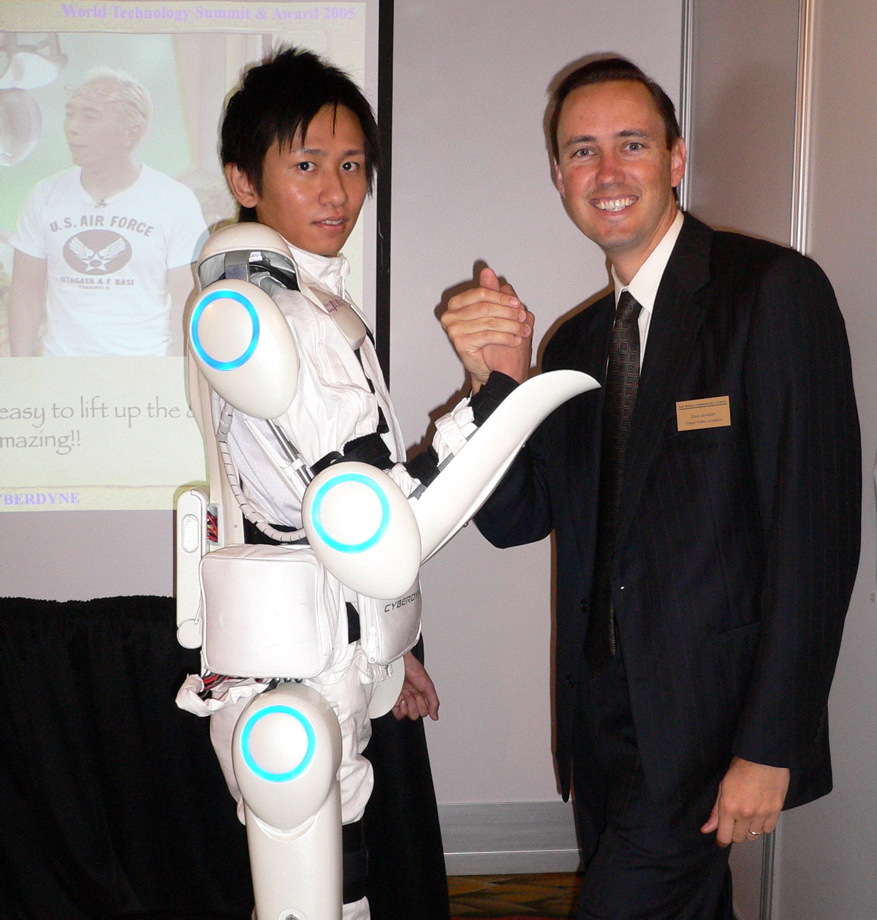
\includegraphics[width=5cm]{P2023.AIBCCSS.ExtendedMindDistributedCognitionSystemicThinking/Hybrid_Assistive_Limb.jpg}
 
 \end{center}
 
\begin{center}
    \tiny{Picture taken from \url{https://en.wikipedia.org/wiki/Powered_exoskeleton}.}
\end{center}
\end{frame}

\begin{frame}
{\centerline{Beliefs}}
\begin{itemize}
    \item The mind is also the center of our beliefs
    \item Typically we think at beliefs as something completely internal to our mind
    \item Is it really so?
    \begin{itemize}
    \item \textcolor{red}{Active Externalism}
\end{itemize} 
     \item Think at exoskeleton, for instance 
\end{itemize} 



\end{frame}



\begin{frame}
{\centerline{Questions?}}
\vspace{1cm}
\begin{center}
    \LARGE{End of lecture six.}
\end{center}

\end{frame}


\end{document}
